% E0240 Project 1, Phase-2 progress report (due 27 October 2026).
% NOTE: the "Group members" line in the title block is a placeholder,
% the same one carried from the Phase-1 statement; fill or delete before
% submission. Every numerical value in this report is traceable to
% Project_Simulator/results/*.csv.
\documentclass[11pt,a4paper]{article}
\usepackage[utf8]{inputenc}
\usepackage[margin=1.5cm,footskip=25pt]{geometry}
\usepackage{amsmath,amssymb}
\usepackage{microtype}
\usepackage{booktabs}
\usepackage{float}
\usepackage{caption}
\captionsetup{font=small,labelfont=bf,skip=4pt}
\usepackage{tikz}
\usetikzlibrary{arrows.meta,positioning,calc}
\usepackage[hidelinks]{hyperref}

\setlength{\parskip}{1.5pt}
\emergencystretch=1em
\makeatletter
\renewcommand\section{\@startsection{section}{1}{\z@}%
  {-3.1ex plus -0.6ex minus -.2ex}{1.6ex plus .2ex}{\normalfont\Large\bfseries}}
\makeatother
\setlength{\intextsep}{4pt plus 1pt minus 1pt}

\title{\vspace{-2.2em}\textbf{\huge E0240: Modeling and Simulation}\\[0.4em]
\Large \textbf{Project Phase-2: Progress Report}\\[0.3em]
\large A Queueing-Network Simulator for an LLM Inference Serving Pipeline}
\author{\textbf{Name:} Vaibhav Mahore \quad \textbf{SR No.:} 23631\\[0.2em]
\textit{UG BTech (M\&C)}, Department of Computer Science and Automation (CSA)\\[0.2em]
\textbf{Indian Institute of Science, Bangalore}\\[0.2em]
\textbf{Group members:} \textit{[Name (SR No.)] \quad [Name (SR No.)]}}
\date{\textbf{Submission Date:} 27 October 2026}

\begin{document}
\maketitle
\vspace{-0.4em}
\hrule
\vspace{1.2em}

\section*{1. Introduction and Problem Definition}
Our project is to collect a queueing network for a real-time system and build a
simulator that captures its key performance metric, queue occupancy. The system
we chose in the Phase-1 statement is an LLM inference serving pipeline: a
request is admitted and tokenized, held by a scheduler until a batch is ready,
and decoded on GPU workers, and at every stage the user-visible latency is
mostly waiting. The serving pipeline is therefore naturally an open queueing
network, and the scheduler settings (batch size, batch wait timer, worker
count) are exactly the knobs a queueing-network simulator lets us sweep
without experimenting on a shared production system.

Since the Phase-1 statement we have completed the simulator and its validation
and are moving into the experiment phase. This report describes how the
simulator is designed, how it maps to the simulation methodology of the
course, and how we validated it against analytical results.

\section*{2. Queueing-Network Model}
\textbf{2.1 System architecture.} We model the pipeline as three stations in a
single path (Figure 1). Requests enter once, are conserved along the path, and
every station therefore sees the same injection rate $\lambda$ (requests per
cycle; one cycle is one scheduler tick). Arrivals are Bernoulli: in each cycle
a request arrives with probability $\lambda$.

\begin{figure}[H]
\centering
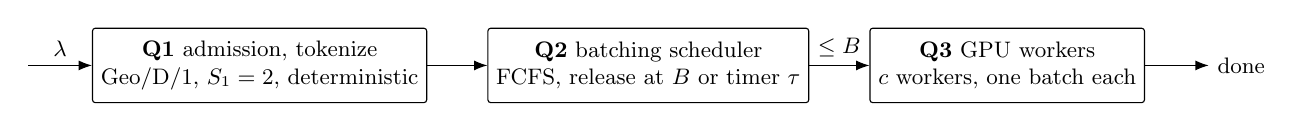
\begin{tikzpicture}[>=Latex, font=\small, scale=0.9, transform shape,
  stn/.style={draw, rounded corners=1pt, minimum width=3.0cm, minimum height=1.05cm, align=center}]
\node[stn] (q1) {\textbf{Q1} admission, tokenize\\ Geo/D/1, $S_1=2$, deterministic};
\node[stn,right=0.85cm of q1] (q2) {\textbf{Q2} batching scheduler\\ FCFS, release at $B$ or timer $\tau$};
\node[stn,right=0.85cm of q2] (q3) {\textbf{Q3} GPU workers\\ $c$ workers, one batch each};
\draw[->] ($(q1.west)+(-0.9,0)$) -- node[above]{$\lambda$} (q1.west);
\draw[->] (q1) -- (q2);
\draw[->] (q2) -- node[above]{$\le B$} (q3);
\draw[->] (q3.east) -- ++(0.9,0) node[right]{done};
\end{tikzpicture}
\caption{The LLM serving pipeline as a three-station queueing network.}
\end{figure}

\textbf{Q1, admission and tokenization} is a single server with deterministic
service $S_1 = 2$ cycles, a Geo/D/1 node whose analytical results carry over
unchanged. \textbf{Q2, the batching scheduler}, is a FCFS release station with
no service: when $B$ requests have collected it releases them as one batch
(this check runs first); otherwise, as soon as the oldest request has waited
$\tau$ cycles, it releases everything then queued as a partial batch. With
$B=1$ or $\tau=0$ the station is a zero-delay pass-through, which is the
configuration we validate against. \textbf{Q3, the GPU workers}, has $c$
identical workers, and one worker serves one \emph{batch}: every request in a
batch shares the batch's service duration and departs when it completes. A
batch of size $b$ has service base $S_3 + \delta(b-1)$, with $S_3 = 2$ and a
configurable batching gain $\delta$; the service law is deterministic
(duration $\lceil S_3 + \delta(b-1)\rceil$ cycles) or geometric (per-cycle
completion at the matching rate, modeling variable decode lengths). $B = 1$
reduces Q3 to ordinary per-request service, which is the form our analytical
anchors take.

\textbf{2.2 Assumptions and parameters.} Each request makes one pass (no
feedback or splits); there is no preemption; workers are identical; batching
changes only how requests wait, apart from the configured batching gain;
arrivals are Bernoulli as above. Node $i$ is stable when
$\rho_i = \lambda_i E[S_i] < 1$, with $\lambda E[S_3]/c$ at Q3. Validation
parameters follow the course sweep: $\lambda \in [0.05{:}0.05{:}0.45,\,0.49]$,
$S \in \{2,3\}$ for the single-station anchors, geometric mean service 2, and
simulation lengths $10^3$, $10^5$ and $10^7$ cycles with a fixed random seed
(20260922) so every run is reproducible.

\section*{3. Simulator Design}
\textbf{3.1 Cycle-driven simulation.} Time advances in fixed increments of one
cycle. This is a deliberate model choice: the system is naturally slotted (one
scheduler tick per cycle), arrivals are Bernoulli per cycle, service
completions are evaluated on cycle boundaries, and queue occupancy is defined
as a time-average over cycles, so fixed-increment advance represents the model
exactly and an event list would add bookkeeping without changing the reachable
states, since every event in this model falls on a tick boundary. We do not
claim generality for this choice over next-event advance; it matches this
system and the course's cycle-driven formulation, and our single-queue update
follows the class MATLAB model statement for statement: arrival, service
countdown, dispatch, counters, in that order, with same-cycle immediate access
(a request arriving at an idle server starts service in its arrival cycle).

\textbf{3.2 Mapping to the simulation components.} The engine is organized
around the discrete-event-simulation components from the course. The
\emph{system state} is the per-station queue contents with per-request
timestamps, the per-worker busy flags, and the remaining service times or
per-cycle completion probabilities. The \emph{simulation clock} is the integer
cycle counter. The \emph{statistical counters} accumulate queue occupancy
(summed over cycles), queue-wait delays, busy-server cycles, and completions.
The \emph{initialization routine} empties all queues, zeroes the counters, and
seeds the random generator. The \emph{timing routine} is the fixed-increment
advance itself; no event queue is needed. The \emph{event routine} is one
update per station per cycle: complete services, route completions to the next
station (or record departures), dispatch idle servers, and release batches.
The \emph{library routine} draws uniform variates from a fixed-seed generator
and applies the inverse transform technique: Bernoulli arrivals from the test
$U \le \lambda$ and geometric service from the per-cycle completion test. The
engine is topology-driven: a configuration is a list of server stations and
batchers, so a single-station configuration reduces the engine exactly to our
validated single-queue simulator.

\textbf{3.3 Metrics.} We use the course definitions throughout. Queue
occupancy $L_q$ is a time average, the occupancy counter divided by the
simulation length, sampled after dispatch and excluding in-service requests.
Delay $D_i$ at a node is the queue wait, the dispatch cycle minus the arrival
cycle, and the per-node average is $(\sum D_i)/n$. Utilization is busy cycles
over total cycles, and throughput is completed requests over simulation time.
As a consistency relation we use $W = L_q/\lambda$ between the measured
waiting time and occupancy.

\section*{4. Validation}
\textbf{Methodology.} We validate against closed forms with course standing,
using a 1\% relative-error criterion at $10^7$ cycles over the stable sweep
$\lambda \le 0.45$, and we present simulation-length convergence before quoting
any number. At $\lambda = 0.49$ ($\rho = 0.98$ for mean service 2) convergence
is slow at $10^7$ cycles (occupancy error 1.1\%); we treat that point as
informational for the criterion rather than as a pass/fail row, consistent
with its long busy periods.

\textbf{4.1 Geo/D/1.} The single-station engine reproduces the course anchor.
The waiting-time relation $W_q = \rho(S-1)/(2(1-\rho))$ and $L_q = \lambda W_q$
match simulation over the whole sweep: the worst occupancy error at
$\lambda \le 0.45$ is 0.75\% at $S=2$ and 0.46\% at $S=3$, and convergence
follows the expected length law (at $\lambda = 0.3$, the error falls from
7.6\% at $10^3$ to 1.8\% at $10^5$ and 0.46\% at $10^7$ cycles; Figure 2).
Extending the sweep to $S=3$ exposed one subtlety: the $L_q$ expression we had
carried over previously, $\lambda^2(S-1)/(1-\lambda S)$, agrees with simulation
only at $S=2$. Deriving the slotted model's waiting-time distribution
ourselves shows that the $W_q$ expression above is the general one and
$L_q = \lambda W_q$ follows exactly in this convention, because each request
contributes one count per queued cycle to the occupancy counter. Table 1
confirms the $S$-general pair at $S=3$ to 0.44\%.

\textbf{4.2 Geo/Geo/1 and the factor-2 check.} With geometric service of mean
2, occupancy matches $L_q = 2\lambda^2/(1-2\lambda)$ with worst error 0.94\%
over $\lambda \le 0.45$, and the simulated Geo/Geo/1 to Geo/D/1 occupancy
ratio stays within 1\% of 2 over the sweep (Figure 3), reproducing the known
factor-2 relationship between the two models at equal mean service.

\textbf{4.3 Pipeline internal-consistency checks.} For the full pipeline we
claim no network-level closed form. Instead we verify the simulator's
accounting and flow behavior: per-node flow balance (departure/arrival ratio
within $3.4\times10^{-7}$ of 1), measured utilization against the offered load
$\rho_i = \lambda_i E[S_i]$ (within 0.11\%), the $W = L_q/\lambda$ relation per
node (agreement to machine precision), the network-level occupancy total
against $\lambda W_{\text{e2e}}$ (within $3.4\times10^{-7}$), and throughput
against $\lambda$ (within 0.11\%). All pass at every tested load.

\begin{table}[H]
\centering\small
\caption{Representative validation results ($10^7$ cycles; full table in the
project package).}
\begin{tabular}{@{}llrrr@{}}
\toprule
Check & Relation & Expected & Simulated & Rel.\ error \\
\midrule
Geo/D/1, $S{=}2$, $\lambda{=}0.45$ & $L_q$ & 2.0250 & 2.0324 & 0.37\% \\
Geo/D/1, $S{=}2$, $\lambda{=}0.30$ & $W_q$ & 0.7500 & 0.7530 & 0.41\% \\
Geo/D/1, $S{=}3$, $\lambda{=}0.30$ & $L_q=\lambda W_q$ & 2.7000 & 2.7118 & 0.44\% \\
Geo/Geo/1, mean 2, $\lambda{=}0.45$ & $L_q$ & 4.0500 & 4.0775 & 0.68\% \\
Occupancy ratio at $\lambda{=}0.45$ & Geo/Geo/1 $:$ Geo/D/1 & 2.0000 & 2.0062 & 0.31\% \\
Pipeline $Q_1$ utilization, $\lambda{=}0.30$ & $\rho_1=\lambda S_1$ & 0.6000 & 0.5997 & 0.06\% \\
\bottomrule
\end{tabular}
\end{table}

\begin{figure}[H]
\centering
\begin{minipage}[t]{0.48\linewidth}
\centering

\includegraphics[width=\linewidth]{figures/fig_e1_validation_geo_d_1.pdf}
\caption{Geo/D/1 validation: occupancy vs injection rate, one curve per
simulation length, against the analytical value ($S=2$).}
\end{minipage}\hfill
\begin{minipage}[t]{0.48\linewidth}
\centering

\includegraphics[width=\linewidth]{figures/fig_v2_factor2.pdf}
\caption{The factor-2 check at $10^7$ cycles: Geo/Geo/1 occupancy is twice
the Geo/D/1 value at equal mean service 2.}
\end{minipage}
\end{figure}

\section*{5. Current Status and Scope}
The simulator, its validation, and the first network experiments are complete
in the same package. As a first load-response experiment we compared the two
Q3 service laws at equal mean and with the same external arrival stream: at
$\lambda = 0.45$, switching Q3 from deterministic to geometric service raises
the mean end-to-end sojourn from 8.52 to 15.35 cycles for one worker, while a
second worker absorbs almost all of the difference (8.55 against 8.52). The
batching experiment, a grid over batch size and wait timer with the
configurable batching gain, is implemented and exercised; we reserve its
analysis for the final report. What is intentionally outside the present
scope: analytical results for interacting stations, which we will add as
validation targets once the corresponding queueing-theory material has been
covered; our current network checks are accounting and flow consistency, not
new theory.

\section*{6. Conclusion}
We have built a cycle-driven, topology-driven queueing-network simulator for
an LLM inference serving pipeline, organized around the simulation components
taught in the course and anchored so that a single-station configuration
reduces it exactly to our validated single-queue models. The engine is
validated against
the discrete-time analytical results for Geo/D/1 and Geo/Geo/1 within the 1\%
criterion at every converged load, including the factor-2 relationship between
the two, and the full pipeline passes the internal flow and accounting checks.
The package is deterministic and one-command reproducible, which puts the
experiment analysis for the final report on a settled footing.

\end{document}
